\documentclass[12pt]{beamer}
\usetheme{Boadilla}
\usepackage[russian]{babel}
\usepackage[utf8]{inputenc}
\usepackage[T2A]{fontenc}
\usepackage[warn]{mathtext}
\usepackage{amsmath}
\usepackage{amssymb}
\usepackage{graphicx}

\title{Динамика демографии, экономика и мигранты}
\subtitle{основные модели популяционной динамики}
\author[Чечулин Артём Владимирович]{
    Автор: Чечулин Артём Владимирович, студент кафедры биоинформатики, группа 302, СПБАУ им. Ж. И. Алферова \\
    Руководитель: Рузин Игорь Мартынович, в.н.с., д. ф.-м.н, ИЭФБ РАН
}
\date{\today}

\begin{document}

\begin{frame}
\titlepage
\end{frame}

\begin{frame}{Содержание}
\tableofcontents
\end{frame}

%% ========================================================================
%% БЛОК 1. ВВЕДЕНИЕ И ПОСТАНОВКА ЗАДАЧ
%% ========================================================================
\section{Введение}

\begin{frame}{Актуальность}

\textbf{Экологическое моделирование является неотъемлемым элементом современной экологии}. Его методы применяются, например, в лесном и сельском хозяйстве.

\textbf{Одной из ключевых задач в этой области является моделирование численности популяций биологических видов}. Получаемые результаты имеют прикладное значение: они могут быть использованы для корректировки мер по сохранению исчезающих и уязвимых видов.

\textbf{Близким экологическому является демографическое моделирование}, где используются модели, адаптированные в соответствии со свойствами человеческих популяций для исследования социально-экономических процессов.

\textbf{Изучению ключевых моделей в этих двух областях} была посвящена значительная часть НИР.

\end{frame}

\begin{frame}{Цель и задачи работы}

\begin{block}{Цель}
исследование моделей взаимодействующих популяций и получение условий их устойчивого сосуществования.
\end{block}

\begin{exampleblock}{Задачи}
\begin{enumerate}
    \item Обзор классических моделей (экспоненциальный рост $\to$ логистический рост $\to$ модель Лотка-Вольтерра).
    \item Исследование границ применимости и аналитическое получение соотношений для моделей.
    \item Реализация моделей в MATLAB.
\end{enumerate}
\end{exampleblock}
\end{frame}

%% ========================================================================
%% БЛОК 2. КЛАССИЧЕСКИЕ МОДЕЛИ (ФУНДАМЕНТ)
%% ========================================================================
\section{Классические модели}

\begin{frame}{Введение. Экспоненциальный рост}

Пусть функция $N(t)$ - численность вида в момент $t$, тогда скорость изменения численности: 

\begin{center}
$\frac{dN}{dt}= births-deaths+migration-emigration.$
\end{center}

В простейшем случае миграцией и эмиграцией пренебрегают; рождаемость и смертность представляются прямо зависящими $N$, разность $(b-d)$ обозначается как чистый темп прироста популяции $r$, и для $ N(t)$ возникает решение вида:

\begin{center}
$\frac{dN}{dt}= bN-dN = rN \implies N(t) = N_0e^{rt}$
\end{center}

\begin{exampleblock}{Характеристики}
\begin{itemize}
    \item рост пропорционален численности;
    \item подходит только при неограниченных ресурсах;
    \item служит базовой моделью для всех последующих.
\end{itemize}
\end{exampleblock}

\end{frame}

\begin{frame}{Логистическая модель}

Идея: скорость размножения популяции пропорциональна её текущей численности и количеству доступных ресурсов.

\[
\frac{dN}{dt}=rN\left(1-\frac{N}{K}\right)
\]

Если $N_0 = N(0)$ (задана начальная численность), то решение следующее:

\begin{center}
$N(t) = \frac{N_0Ke^{rt}}{[K+N_0(e^{rt}-1)]} \to K$ при $t \to \infty$
\end{center}

\begin{exampleblock}{Характеристики}
\begin{itemize}
    \item рост ограничен ёмкостью среды $K$;
    \item устойчиво выходит на стационар $N=K$.
\end{itemize}
\end{exampleblock}

\end{frame}

\begin{frame}{Тип динамики численности зависит от $N_0$}
\begin{figure}
    \centering
    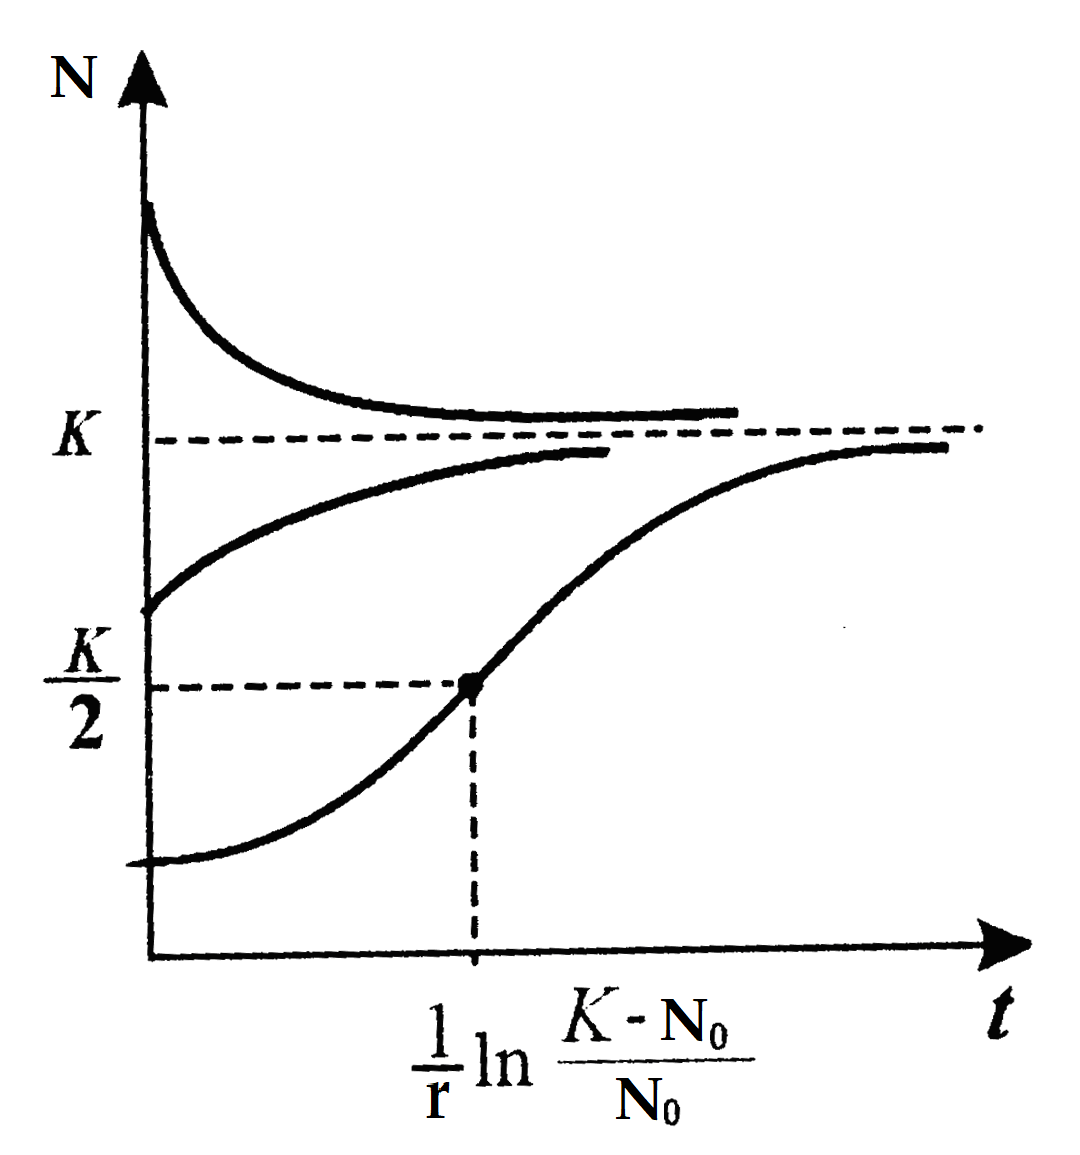
\includegraphics[width=0.45\linewidth]{3_ways.png}
    \caption{Варианты динамики: 1) $N_0 > K$; 2) $K > N_0 > \frac{K}{2}$; 3) $N_0 < \frac{K}{2}$.}
\end{figure}
\end{frame}

%% ========================================================================
%% БЛОК 3. МОДЕЛЬ НЕФЕДОВА — С ПОЯСНЕНИЯМИ
%% ========================================================================

\begin{frame}{Аграрная модель}

Логистическое уравнение хорошо описывает замедление роста, но не объясняет спады численности. В реальных популяциях (и человеческих обществах) наблюдаются колебания — их часто объясняют внешними причинами (войны, эпидемии, климат).

\begin{block}{Гипотеза}
В земледельческом обществе колебания могут быть внутренними (эндогенными), если ёмкость среды $K$ не постоянна, а зависит от урожая, который собирают сами люди.
\end{block}

Для аграрном обществ ёмкость среды $K$ — это запасы, например, зерна (в пайках), которые могут прокормить население.

\end{frame}

\begin{frame}{Переменная ёмкость среды}

\begin{block}{Уравнения модели}
\[
\begin{cases}
\displaystyle \frac{dN}{dt} = rN\left(1-\dfrac{N}{K}\right) \\[14pt]
\displaystyle \frac{dK}{dt} = P(N) - N
\end{cases}
\]
\end{block}

Здесь:
\begin{itemize}
    \item $N$ — численность населения,
    \item $K$ — запасы зерна (ёмкость среды в данный момент),
    \item $P(N)$ — годовой урожай (в пайках),
    \item $r$ — темп роста населения ($0.01 < r < 0.02$).
\end{itemize}

Уравнение для $K$: запасы растут, если урожай превышает потребление ($N$ пайков в год), и падают в противном случае.

\end{frame}

\begin{frame}{Функция урожая}

Урожай $P(N)$ должен учитывать два ограничения:
\begin{itemize}
    \item При малом $N$ главный лимит — рабочие руки (урожай растёт пропорционально $N$).
    \item При большом $N$ — земля (урожай насыщается).
\end{itemize}

Простейшая функция с такими свойствами:
\[
P(N) = \frac{aN}{N+d}
\]

\begin{exampleblock}{Смысл параметров}
\begin{itemize}
    \item $a$ — максимальный урожай (когда вся земля засеяна),
    \item $d$ — масштаб насыщения: при $N = d$ используется $\frac{1}{2}$ земли,
    \item $q = \dfrac{a}{d}$ — продуктивность труда (сколько человек кормит один земледелец в благоприятных условиях).
\end{itemize}
\end{exampleblock}

\end{frame}

\begin{frame}{Продуктивность земледелия}

При малом населении ($N \ll d$):
\[
P(N) \approx \frac{a}{d} N = qN
\]

То есть один работник производит $q$ пайков. Исторические оценки для традиционного сельского хозяйства:
\[
1.2 < q < 2
\]
(земледелец кормит себя и ещё максимум одного человека).

При большом населении ($N \gg d$):
\[
P(N) \to a
\]
— урожай упирается в земельный лимит.

\end{frame}

\begin{frame}{Стационарные состояния}

Ищем точки, где население и запасы не меняются:
\[
\frac{dN}{dt}=0,\quad \frac{dK}{dt}=0.
\]

\begin{itemize}
    \item Из $\frac{dN}{dt}=0$ при $N>0$ получаем: $N = K$.
    \item Из $\frac{dK}{dt}=0$: $\displaystyle \frac{aN}{N+d} - N = 0$.
\end{itemize}

Решаем второе уравнение:
\[
\frac{a}{N+d} = 1 \quad\Rightarrow\quad a = N + d \quad\Rightarrow\quad N_0 = a - d.
\]

Так как $N = K$, то равновесие:
\[
N_0 = K_0 = a - d \quad (\text{при } a > d).
\]
\end{frame}

\begin{frame}{Цикл в аграрной модели}

Почему возникают циклы? 

\centering
\begin{exampleblock}{}
\[
\boxed{N \uparrow} 
\xrightarrow{\text{больше работников}} 
\boxed{P \uparrow} 
\xrightarrow{\text{больше еды}} 
\boxed{K \uparrow} 
\xrightarrow{\text{можно больше людей}} 
\boxed{N \uparrow}
\]
\vspace{0.1cm}
\[
\downarrow
\]
\vspace{0.1cm}
\[
\boxed{P\text{ насыщается}} 
\xrightarrow{\text{инерция}} 
\boxed{N \uparrow}
\xrightarrow{\text{превышает K}} 
\boxed{N > K}
\xrightarrow{\text{запасы тают}}
\boxed{K \downarrow}
\]
\vspace{0.1cm}
\[
\downarrow
\]
\vspace{0.1cm}
\[ 
\xrightarrow{\text{голод}} 
\boxed{N \downarrow} 
\xrightarrow{\text{земля опустевает}} 
\boxed{P \ \text{снова может} \uparrow} 
\xrightarrow{\text{}} 
\boxed{K \uparrow} 
\xrightarrow{\text{повтор}} 
\boxed{N \uparrow}
\]
\end{exampleblock}

\end{frame}

\begin{frame}{Демографические циклы}

Параметры: $r = 0.015$, $N_0 = 100$, $K_0 = 50$, $q = \dfrac{a}{d} = \dfrac{650}{500} = 1.3$.

\begin{figure}[H]
    \centering
    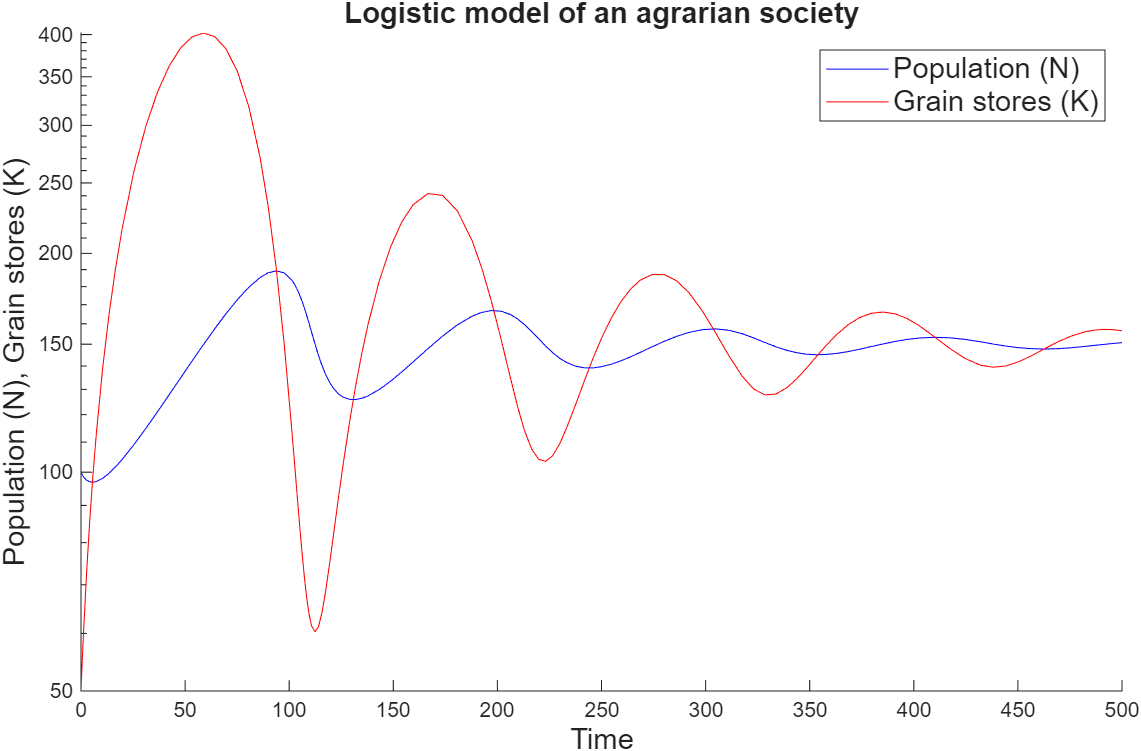
\includegraphics[width=0.65\linewidth]{log_agrar.png}
\end{figure}

Амплитуда уменьшается, циклы стабилизируются — система выходит на равновесие через затухающие колебания.

\end{frame}

\begin{frame}{Демографическая катастрофа}

Параметры: $r = 0.02, a = 130, d = 100, N_0 = 50, K_0 = 200.$

\begin{figure}[H]
    \centering
    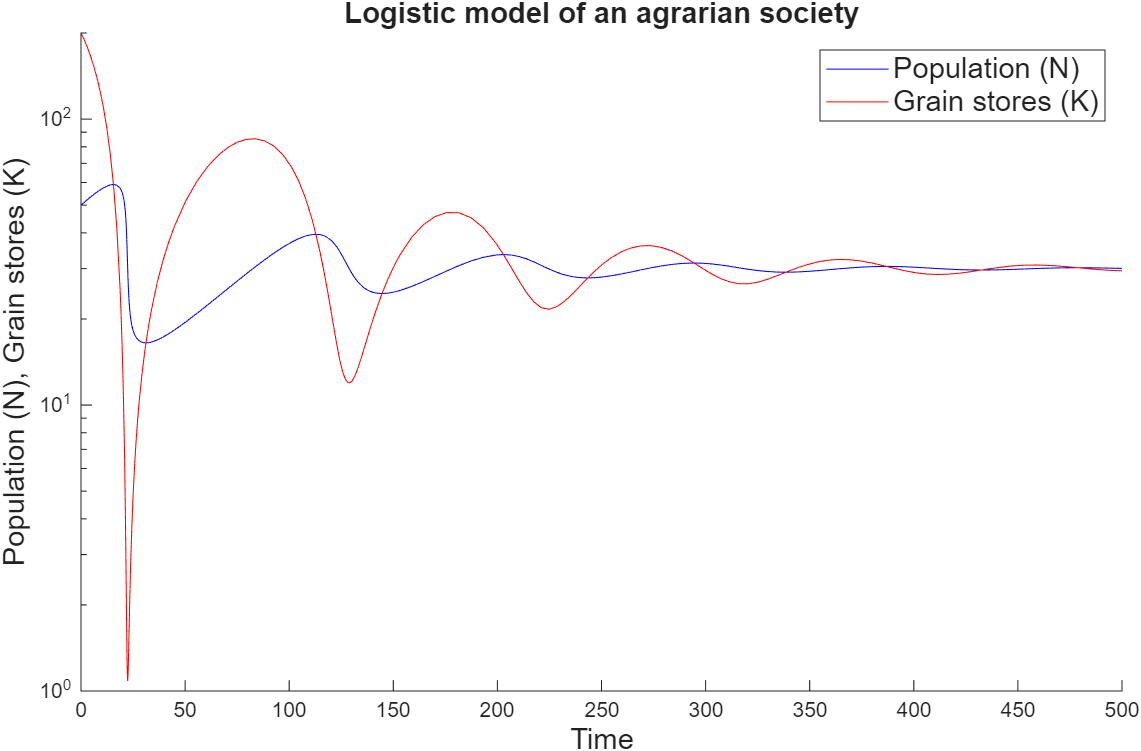
\includegraphics[width=0.65\linewidth]{dem_cat.png}
\end{figure}

Взят большой $r$. Население продолжает расти, когда ресурс уже сокращается — запаздывание реакции. Оно приводит к падению численности в разы ввиду уменьшения ёмкости среды $K(t)$.

\end{frame}

\begin{frame}{От аграрной модели — к хищник–жертва}

В аграрной модели мы рассматривали общество, где население само производит и потребляет ресурс.

\begin{exampleblock}{Обобщение}
\begin{itemize}
    \item Ресурс — то, что потребляется
    \item Потребитель — тот, кто потребляет ресурс
    \item Между ними — обратная связь
\end{itemize}
\end{exampleblock}

Та же логика работает в экологии:

\begin{itemize}
    \item Ресурс — жертва (трава, зайцы)
    \item Потребитель — хищник (рыси)
    \item Хищники не производят ресурс, а только потребляют
    \item Но математическая структура похожа: 
    \[
    \begin{cases}
    \frac{dC}{dt} = \text{прирост} - \text{потребление} \\
    \frac{dH}{dt} = \text{рождаемость} - \text{смертность}
    \end{cases}
    \]
\end{itemize}

\end{frame}

%% ========================================================================
%% БЛОК 4. МОДЕЛИ ХИЩНИК-ЖЕРТВА
%% ========================================================================
\section{Модель <<хищник-жертва>>}

\begin{frame}{Модель <<хищник-жертва>>}

Модель Лотка-Вольтерра - это один из самых известных биологических циклов. Хищник питается жертвой, жертва размножается, и их популяции колеблются. Модель описывает качественный механизм изменения численностей, но имеет особенность: равновесие типа «центр», а это означает, что колебания численностей не затухают, но и не нарастают.

\[
\begin{cases}
\frac{dC}{dt}=aC-bCH\\
\frac{dH}{dt}=cCH-dH
\end{cases}
\]

\begin{exampleblock}{Характеристики}
\begin{itemize}
    \item система неустойчива к малым изменениям;
    \item неизменные колебания численности.
\end{itemize}
\end{exampleblock}

\end{frame}

\begin{frame}{Расчёт и реальное изменение численности}
\begin{figure}
    \centering
    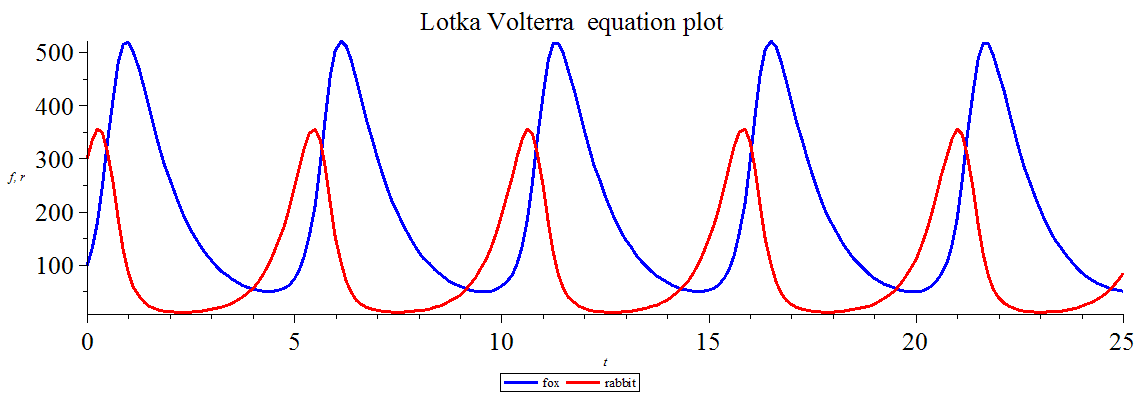
\includegraphics[width=0.6\linewidth]{LV_test.png}
\end{figure}
\begin{figure}
    \centering
    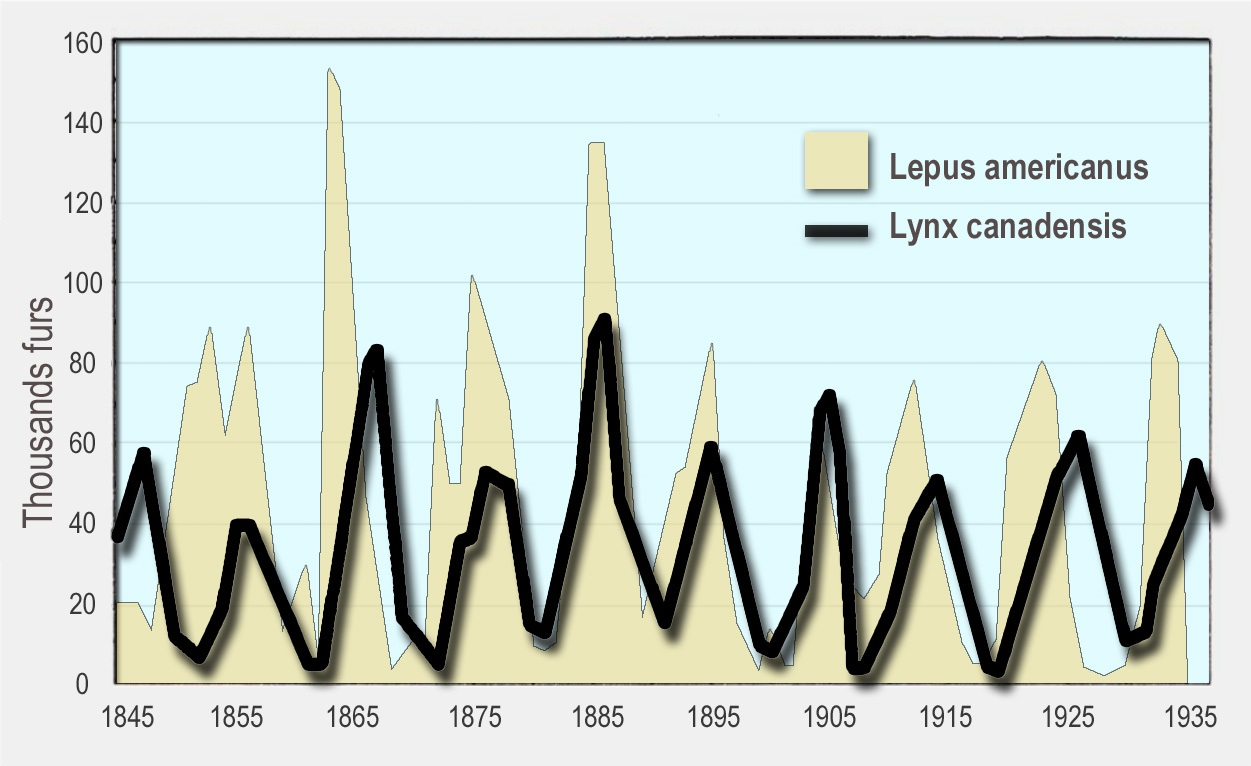
\includegraphics[width=0.6\linewidth]{LYNX.jpg}
\end{figure}
\end{frame}

\begin{frame}{Асимметричная пищевая цепочка}
\begin{figure}
    \centering
    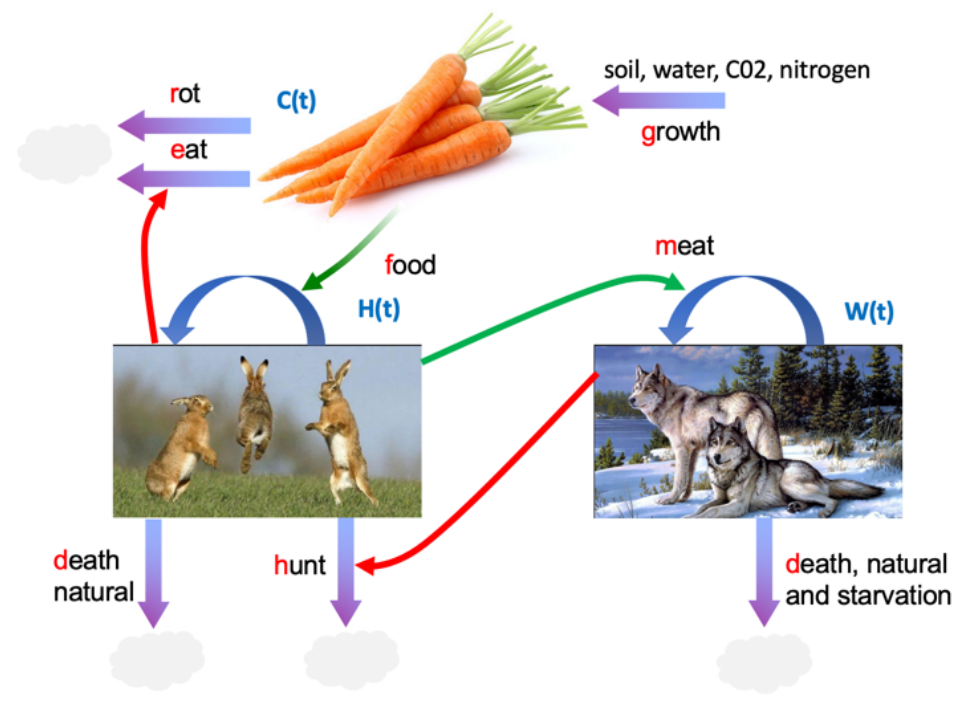
\includegraphics[width=0.75\linewidth]{LVscheme.png}
    \caption{Схема измененной модели Лотка-Вольтерра}
\end{figure}
\end{frame}

\begin{frame}{Собственная динамика ресурса улучшает модель}

Проблема классической Лотки-Вольтерра в том, что ресурс $C$ не имеет собственной динамики, кроме поедания его хищником, и ввиду этого система не имеет устойчивого равновесия. Решение: добавляем ресурсу собственную динамику — постоянный приток $g$ и естественную убыль $r$. 

\begin{block}{Улучшенная модель}
\[
\begin{cases}
\frac{dC}{dt}=g-(r+eH)C \\
\frac{dH}{dt}=H(fC-d_H)
\end{cases}
\]
\end{block}

Найдём стационарное состояние - такую точку $(C_0, H_0)$, где обе популяции не меняются.

\end{frame}

\begin{frame}{Находим стационарное состояние}

Из $\frac{dH}{dt}=0$ при $H>0$:
\[fC - d_H = 0 \quad \Rightarrow \quad C_0 = \frac{d_H}{f}\]

Это уровень ресурса, при котором $H$ не меняется. Подставляем $C_0$ в $\frac{dC}{dt}=0$:
\[g - (r + eH_0)C_0 = 0 \quad \Rightarrow \quad g = rC_0 + eH_0C_0\]

Выражаем $H_0$:
\[H_0 = \frac{g - rC_0}{eC_0} = \frac{g - r\frac{d_H}{f}}{e\frac{d_H}{f}} = \frac{1}{e} \left(\frac{gf}{d_H} -r\right) = \frac{r}{e}\left(\frac{g f}{r d_H} - 1\right)\]

\end{frame}

\begin{frame}{Соотношение для $H_0$}

Получим компактное выражение для $H_0$:
\[R_0 = \frac{g f}{r d_H}\ \implies H_0 = \frac{r}{e}(R_0 - 1)\]

\begin{exampleblock}{Коэффициент воспроизводства $R_0$}
Это число потомков, произведённых особью за время жизни:
\begin{itemize}
\item $R_0 > 1$ — популяция растёт
\item $R_0 = 1$ — стабильна
\item $R_0 < 1$ — вымирает
\end{itemize}
\end{exampleblock}

$gf$ — кол-во ресурса, которое преобразуется в потомство, а $rd_H$ — смертность. Анализ устойчивости показывает, что точка равновесия $(C_0, H_0)$ асимптотически устойчива при $R_0 > 1$.

\end{frame}

%% ========================================================================
%% БЛОК 5. ОРИГИНАЛЬНАЯ ЧАСТЬ: МОДЕЛЬ С МИГРАНТАМИ — С ПОЯСНЕНИЯМИ
%% ========================================================================
\section{Модель с постоянным потоком мигрантов}

\begin{frame}{Две популяции и один ресурс}

Демографический вариант модели Лотка-Вольтерры. Система: ресурс ($C$), местная популяция ($H$), внешняя популяция ($M$).

\begin{block}{Система уравнений}
\[
\begin{cases}
\frac{dC}{dt} = g - (r + e_H H + e_M M)C \\[12pt]
\frac{dH}{dt} = H(f_H C - d_H) \\[12pt]
\frac{dM}{dt} = M(f_M C - d_M) + \mu
\end{cases}
\]
где:
\begin{itemize}
    \item $g$ — постоянный приток ресурса (например, урожай),
    \item $r$ — естественная убыль ресурса (например, гниение),
    \item $\mu$ — миграционный поток (число прибывающих в единицу $t$).
\end{itemize}
\end{block}

Найдём стационарные условия.

\end{frame}

\begin{frame}{Случай без потока ($\mu = 0$)}

Из $\frac{dH}{dt}=0$, $\frac{dM}{dt}=0$ при $H>0$, $M>0$:
\[f_H C - d_H = 0, \quad f_M C - d_M = 0\]

Отсюда:
\[C = \frac{d_H}{f_H} = \frac{d_M}{f_M}\]

\begin{block}{Условие сосуществования}
\[\frac{d_H}{f_H} = \frac{d_M}{f_M}\]
\end{block}

Сосуществование в данной модели требует точного равенства параметров. Это равенство  — случайность, в реальности оно почти никогда не выполняется, и одна популяция вытесняет другую (принцип конкурентного исключения).

\end{frame}

\begin{frame}{Вывод условий для случая с потоком ($\mu > 0$)}

Из $\frac{dH}{dt}=0$, $H>0$:
\[f_H C - d_H = 0 \quad \Rightarrow \quad C = \frac{d_H}{f_H}\]

Это означает: в равновесии ресурс фиксирован на уровне, необходимом локальной популяции для выживания.

Из $\frac{dM}{dt}=0$:
\[M(f_M C - d_M) + \mu = 0 \quad \Rightarrow \quad M = \frac{\mu}{d_M - f_M C}\]

Подставляем $C$:
\[M = \frac{\mu}{d_M - f_M \frac{d_H}{f_H}}\]

\end{frame}

\begin{frame}{Условие положительности $M$}

Чтобы $M > 0$, знаменатель должен быть положительным (так как $\mu>0$):
\[d_M - f_M \frac{d_H}{f_H} > 0\]

Переносим:
\[d_M > \frac{f_M d_H}{f_H} \quad \Leftrightarrow \quad \frac{d_M}{f_M} > \frac{d_H}{f_H}\]

\begin{exampleblock}{Смысл}
Отношение $\frac{d}{f}$ — это уровень ресурса, необходимый для выживания. 
Чем оно меньше, тем эффективнее популяция расходует ресурс. 
Условие $\frac{d_M}{f_M} > \frac{d_H}{f_H}$ означает, что внешняя популяция менее эффективна, чем локальная.
\end{exampleblock}

Без этого условия равновесие с $M>0$ просто не существует.

\end{frame}

\begin{frame}{Находим $H$ из уравнения ресурса}

Из $\frac{dC}{dt}=0$:
\[g - (r + e_H H + e_M M)C = 0\]

Подставляем $C = \frac{d_H}{f_H}$:
\[g - r\frac{d_H}{f_H} - e_H H \frac{d_H}{f_H} - e_M M \frac{d_H}{f_H} = 0\]

Выражаем $H$:
\[H = \frac{1}{e_H}\left(\frac{g f_H}{d_H} - r - e_M M\right)\]

\end{frame}

\begin{frame}{Появление $R_0$}

Заметим, что выражение $\frac{g f_H}{d_H} - r$ можно переписать через уже знакомый нам коэффициент воспроизводства локальной популяции:
\[R_0 = \frac{g f_H}{r d_H}\quad\Longrightarrow\quad \frac{g f_H}{d_H} - r = r(R_0 - 1)\]

Тогда формула для $H$ принимает компактный вид:
\[H = \frac{1}{e_H}\bigl(r(R_0 - 1) - e_M M\bigr)\]

Условие существования локальной популяции ($H>0$) теперь выглядит как:
\[e_M M < r(R_0 - 1)\]

\end{frame}

\begin{frame}{Подставляем $M$}

\[M = \frac{\mu}{d_M - f_M \frac{d_H}{f_H}}\]

Получаем:
\[H = \frac{1}{e_H}\left(r(R_0 - 1) 
      - e_M \frac{\mu}{d_M - f_M \frac{d_H}{f_H}}\right)\]

Условие $H > 0$:
\[r(R_0 - 1) - e_M 
      \frac{\mu}{d_M - f_M \frac{d_H}{f_H}} > 0\]

Это ограничение на поток: если он слишком велик, численность локальной популяции уходит в ноль.

\end{frame}

\begin{frame}{Критический поток}

Переносим:
\[e_M \frac{\mu}{d_M - f_M \frac{d_H}{f_H}} < r(R_0 - 1)\]

Домножаем:
\[\mu < \frac{1}{e_M}\, r(R_0 - 1)\left(d_M - \frac{f_M d_H}{f_H}\right)\]

\begin{exampleblock}{Условие $H > 0$}
\[\mu < \mu_{\text{crit}}\]
где 
\[\mu_{\text{crit}} = \frac{r}{e_M}(R_0 - 1)\left(d_M - \frac{f_M d_H}{f_H}\right) > 0.\]
\end{exampleblock}

\end{frame}

\begin{frame}{Интерпретация полученных условий}

\begin{block}{Условие 1}
\[\frac{d_M}{f_M} > \frac{d_H}{f_H}\]
Внешняя популяция должна менее эффективно использовать ресурс, чем локальная. Иначе малый поток вытесняет местную популяцию.
\end{block}

\begin{block}{Условие 2}
\[\mu < \mu_{\text{crit}}\]
Миграционный поток не должен превышать критический порог.
\end{block}

При выполнении обоих условий сосуществование возможно в целой области параметров, а не только в точке равенства эффективностей!

\end{frame}

\begin{frame}{Потеря устойчивости}

\begin{block}{Исходная ситуация}
Стационарное состояние одиночной популяции устойчиво при $R_0 > 1$.
\end{block}

\begin{exampleblock}{Добавляем мигрантов ($\mu > 0$)}
\begin{itemize}
    \item Если $\frac{d_M}{f_M} < \frac{d_H}{f_H}$ (внешняя популяция эффективнее) 
          — даже малый $\mu$ вытесняет местную популяцию.
    \item Если $\frac{d_M}{f_M} > \frac{d_H}{f_H}$ (внешняя популяция менее эффективна), 
          но $\mu > \mu_{\text{crit}}$ — локальная популяция вымирает.
\end{itemize}
\end{exampleblock}

Таким образом, даже малый, но постоянный поток мигрантов может разрушить равновесие, если он превышает $\mu_{\text{crit}}$.

\end{frame}

\begin{frame}{Превышение критического порога}

Параметры: 
$H_0 = 1000$, $M_0 = 0$, $\frac{d_H}{f_H} = 4$, $\frac{d_M}{f_M} = 4.5$, $g = 5$, $r = 0.1$, $\mu = 17$. Сначала система находится в равновесии с популяцией $H$, а в момент $t = 10$ начинается постоянный приток $\mu$.

\begin{figure}[H]
    \centering
    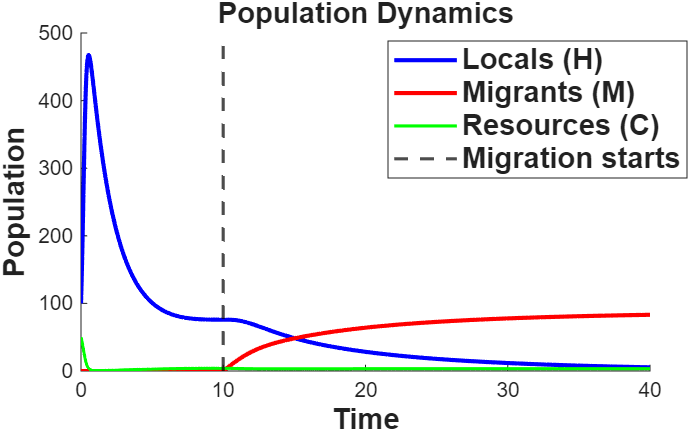
\includegraphics[width=0.6\linewidth]{p5.1.png}
\end{figure}

Внешняя популяция менее эффективно использует ресурс, но $\mu_{\text{crit}} \approx 7.67 < 17$, поэтому $H \to 0$.

\end{frame}

%% ========================================================================
%% БЛОК 6. ЗАКЛЮЧЕНИЕ
%% ========================================================================

\section{Заключение}

\begin{frame}{Результаты и выводы}

\begin{exampleblock}{Основные результаты}
\begin{enumerate}
    \item Получены аналитические условия сосуществования для модели с постоянным миграционным потоком:
    \[
    \frac{d_M}{f_M} > \frac{d_H}{f_H}, \quad \mu < \mu_{\text{crit}}
    \]
    \item Рассмотрен эффект потери устойчивости одиночной популяции при добавлении внешней.
\end{enumerate}
\end{exampleblock}

Классические модели требуют модификации для описания демографических процессов.

\end{frame}
\begin{frame}{Спасибо за внимание!}
\begin{center}
\Huge Вопросы?
\end{center}
\end{frame}

\begin{frame}{Реализация модели в MATLAB}

\begin{figure}[H]
    \centering
    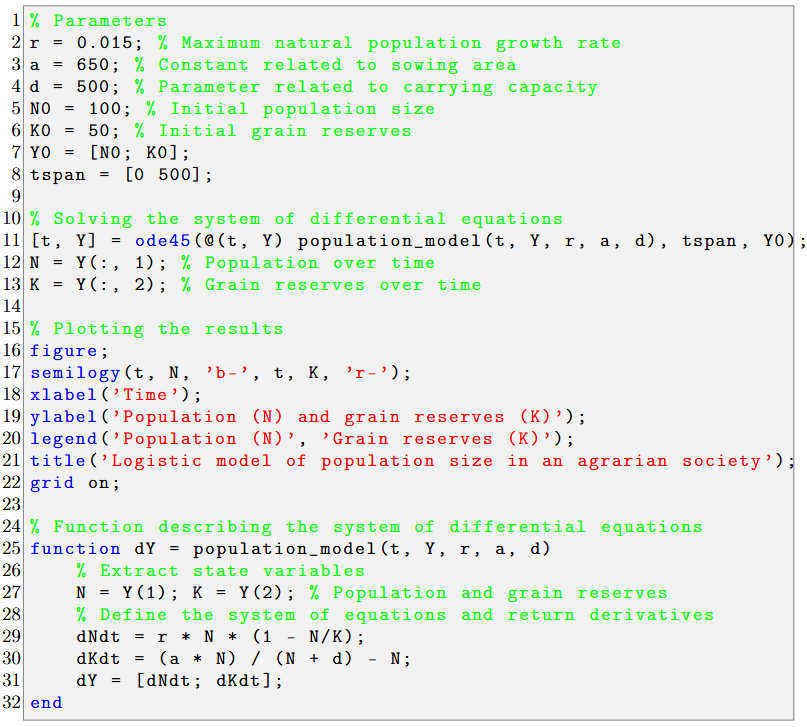
\includegraphics[width=0.75\linewidth]{code.png}
\end{figure}

\end{frame}

\begin{frame}{Возмущение переводит на иную траекторию}
\begin{figure}
    \centering
    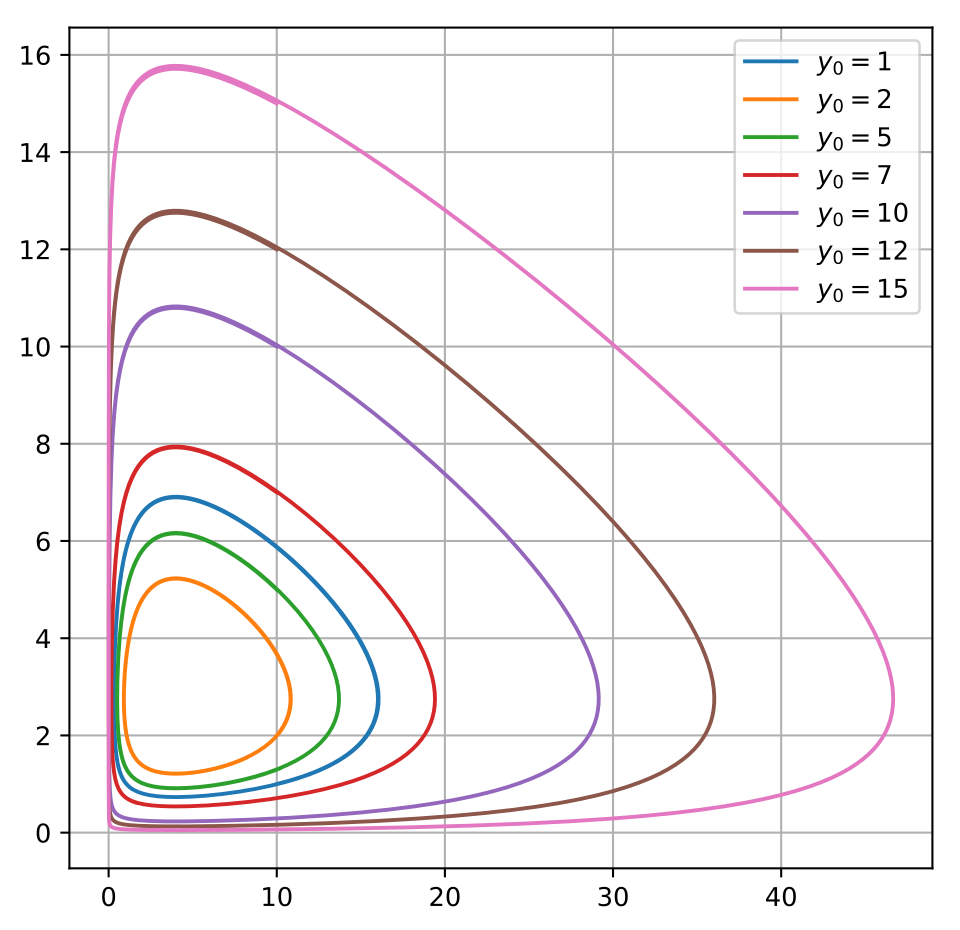
\includegraphics[width=0.6\linewidth]{dynamics.png}
    \caption{Фазовый портрет системы для разных начальных количеств $y_0$}
\end{figure}
\end{frame}

\begin{frame}{Анализ устойчивости и линеаризация}

Теперь проверяем, будет ли система возвращаться в равновесие после малых отклонений. Вводим возмущения:
\[C(t) = C_0 + C'(t), \quad H(t) = H_0 + H'(t)\]

Линеаризуем систему — раскладываем правые части в ряд Тейлора (как ф-ии двух переменных $F(C, H), \ G(C,H)$), оставляя только линейные члены. Посчитав частные производные по переменным, вычисленным в равновесии, получим:

\begin{block}{Матрица Якоби}
\[J = \begin{bmatrix} -r + eH_0 & -eC_0 \\ fH_0 & 0 \end{bmatrix}\]
\end{block}

\end{frame}

\begin{frame}{Характеристическое уравнение}

Чтобы определить вид устойчивости, ищем собственные значения $\lambda$ из уравнения $\det(J - \lambda I)=0$:

\[\det \begin{bmatrix} -r + eH_0 - \lambda & -eC_0 \\ fH_0 & -\lambda \end{bmatrix} = 0\]

Раскрываем определитель:
\[(-r + eH_0 - \lambda)(-\lambda) - (-eC_0)(fH_0) = 0\]

Получаем:
\[\lambda^2 + (r + eH_0)\lambda + e f C_0 H_0 = 0\]

\end{frame}

\begin{frame}{Анализ корней}

Квадратное уравнение:
\[\lambda^2 + (r + eH_0)\lambda + e f C_0 H_0 = 0\]

\begin{block}{Коэффициенты}
\begin{itemize}
\item $r + eH_0 > 0$ всегда
\item $e f C_0 H_0 > 0$ при $H_0 > 0$ (то есть при $R_0 > 1$)
\end{itemize}
\end{block}

\begin{exampleblock}{Критерий устойчивости}
Если все коэффициенты $> 0$, то либо оба корня отрицательные, либо комплексные с отрицательной действительной частью.
\end{exampleblock}

Значит, точка $(C_0, H_0)$ устойчива при $R_0 > 1$. 

\end{frame}

\end{document}